\chapter{Direzioni future di ricerca e conclusioni}
\label{conclusioni}
\thispagestyle{empty}

%Si mostrano le prospettive future di ricerca nell'area dove si \`e svolto il lavoro. Talvolta questa sezione pu\`o essere l'ultima sottosezione della precedente. Nelle conclusioni si deve richiamare l'area, lo scopo della tesi, cosa \`e stato fatto,come si valuta quello che si \`e fatto e si enfatizzano le prospettive future per mostrare come andare avanti nell'area di studio.

\noindent 
L'obiettivo di questo progetto è creare un simulatore che permetta all'utente di pedalare ed immedesimarsi in un mondo virtuale. I risultati ottenuti nel tentativo di realizzare questo sistema sono discreti, ma non tanto realistici quanto voluto.
Per quanto possa essere accessibile, l'OSVR ha prestazioni piuttosto ridotte se viene utilizzato con ambientazioni con molti dettagli. Per la realtà virtuale è necessario un computer con elevate prestazioni e un visore con un'ottima risoluzione. Per la realizzazione del progetto non è stato possibile utilizzare strumenti con prestazioni migliori e senza questi, i risultati che si ottengono sono simulazioni non molto realistiche e spesso fastidiose. Infatti dopo diverse ore l'utente può accusare affaticamento alla vista, stanchezza e nello specifico cefalea e nausea.\\
Un altro problema è dovuto alla cyclette e al fatto che i dati ricavati dal suo utilizzo siano poco realistici. Non è infatti possibile fermare i piedi sui pedali affidandosi all'inerzia come in una reale bicicletta, poiché la cyclette ha i pedali direttamente ancorati al sistema del volano. Fermare i piedi sulla cyclette porta a fermare direttamente il volano, ma l'applicazione genera comunque l'inerzia sulla bicicletta virtuale. Inoltre, se nel modello vi fosse una salita, la bicicletta virtuale salirebbe più lentamente, ma l'utente che utilizza la cyclette non avrebbe nessun ritorno di forza dovuto alla pendenza.

\section{Soluzione}
Per sopperire a questi due problemi è in corso la progettazione di un sistema più sofisticato, che fa uso di una bicicletta vera e di rulli che permettano di dare un ritorno di forza in caso di pendenze. Un esempio è quello in figura.
 \begin{figure}[htb]
    \centering
    %\vspace{-0.7cm}
    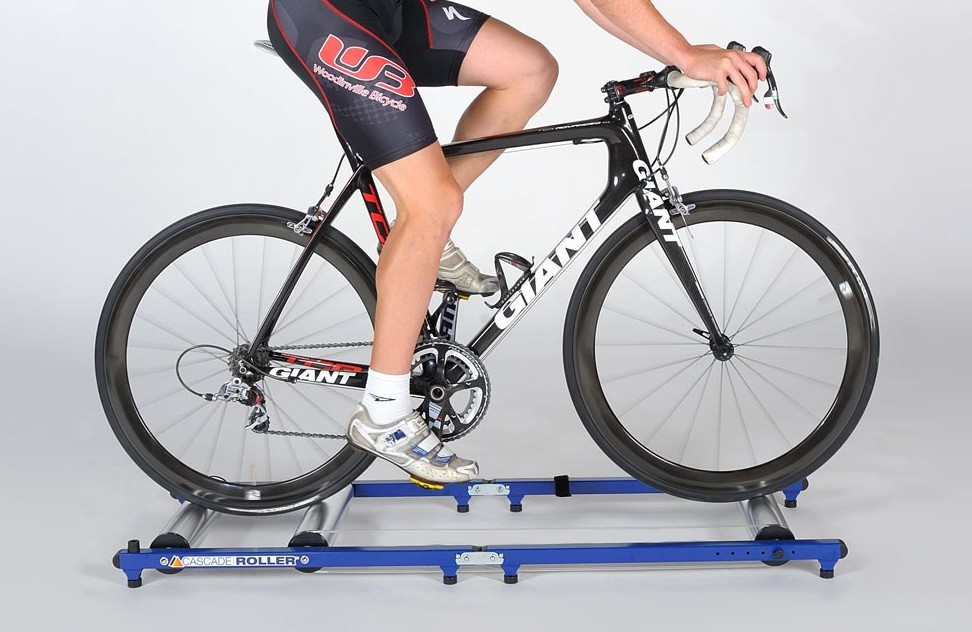
\includegraphics[height=8cm]{biciconrulli}
    \caption{Un esempio di bicicletta con rulli\label{fig:biciconrulli}}
    %\vspace{-0.3cm}
\end{figure}

\noindent Questi rulli avranno un modulo bluetooth che comunicherà con il calcolatore e riceverà da esso delle informazioni sulla pendenza del modello 3D. Inoltre, in futuro il sistema verrà aggiornato con visore molto più sofisticato: l'Oculus Rift. Questo visore ha una risoluzione più elevata e garantisce un'esperienza utente molto più realistica dell'OSVR. Tuttavia, necessita un computer con prestazioni molto più elevate. Verrà infatti installata, nel computer in laboratorio, una scheda video ASUS Strix NVidia GeForce GTX 1080, che è VR Ready, ovvero pronta per poter supportare la realtà virtuale e portare l'esperienza utente ai massimi livelli. Grazie alla popolarità di Unity, l'Oculus Rift è perfettamente integrabile ed esistono pacchetti che permettono di farlo con grande facilità.
\newpage
\section{Conclusioni}
Durante la progettazione, il lavoro è stato svolto con un occhio di riguardo alle future implementazioni. Si è quindi mantenuto un profilo generale anche nei dettagli, che permettesse una facile integrazione di una bicicletta vera. Nonostante la inevitabile eliminazione o variazione di tutto ciò che riguarda la cyclette e l'hardware associato, il simulatore software è già pronto per essere riutilizzato nel sistema con i rulli. L'unica modifica, di facile realizzazione, sarà quella di modificare la velocità in base alle informazioni che il sistema hardware fornirà riguardo alla pendenza. 
Gli sviluppi futuri e le integrazioni che si stanno applicando, porteranno il simulatore ad un livello di realismo considerevole, il quale potrà contribuire a portare la realtà virtuale nella vita di tutti i giorni.
